



%%%%%%%%%%%%%%%%%%%%%%%%%%%%%%%%%%%%%%%%%%%%%%%%%%%
\section{Datasets Used}
\label{sec:DatasetsImplementation}
%%%%%%%%%%%%%%%%%%%%%%%%%%%%%%%%%%%%%%%%%%%%%%%%%%%

For running the experiments, we used datasets that are highly used in the literature, namely the Breast Cancer Wisconsin dataset\footnote{\url{https://archive.ics.uci.edu/ml/datasets/Breast+Cancer+Wisconsin+(Diagnostic)}}, the Pima Indians Diabetes dataset\footnote{\url{https://archive.ics.uci.edu/ml/datasets/pima+indians+diabetes}}, the Credit Approval dataset\footnote{\url{http://archive.ics.uci.edu/ml/datasets/credit+approval}}, and the Adult Income dataset \footnote{\url{https://archive.ics.uci.edu/ml/datasets/adult}}. Table \ref{table:datasets} presents a brief description of each dataset.

\begin{table}[H]
\centering
\caption{Datasets used in \ac{BARD}.}
\label{table:datasets}
\begin{tabular}{|l|l|l|l|}
\hline
\textbf{Dataset} & \textbf{Subject} & \textbf{Instances} & \textbf{Features} \\ \hline
 Breast Cancer Wisconsin  &  HealthCare  & 569    & 30       \\ \hline
 Pima Indians Diabetes    &  HealthCare  & 768    &  8       \\ \hline
 Credit Approval          &  Finance     & 690    & 15       \\ \hline
 Adult Income             &  Governance  & 48842  & 14       \\ \hline 
\end{tabular}
\end{table}



%%%%%%%%%%%%%%%%%%%%%%%%%%%%%%%%%%%%%%%%%%%%%%%%%%%
\section{Data Preprocessing}
\label{sec:DataPreProcessingImplementation}
%%%%%%%%%%%%%%%%%%%%%%%%%%%%%%%%%%%%%%%%%%%%%%%%%%%

Although our data is obtained from publicly available data sources, it is still required to do some preprocessing on the data.
For example, the datasets contained missing values on some of the entries that needed to be addressed. Another example is the existence of categorical data that \ac{ML} algorithms cannot process. We now describe some of the techniques we used in the data preparation phase for the datasets described in Table \ref{table:datasets}.

\begin{itemize}
    \setlength\itemsep{1em}

	\item\textbf{One-hot Encoding}\cite{harris2010digital} was initially used in digital circuits in order to determine the state of a state machine without using a decoder. The binary code is converted in a group of bits in which only one bit can have the value high ($1$), and all the others low ($0$). For example, the binary $110$ is converted to $01000000$.
	In \ac{ML}, we apply this technique to deal with the problems created by using datasets with categorical (or nominal) data. Most \ac{ML} algorithms require numerical representations in the data. A solution can be to assign an integer number to each different value present in the data, but this leads to the model assuming a natural ordering between categories that may not exist.
	Using one-hot encoding in categorical data allows us to circumvent this problem, creating additional binary variables for each unique value, \textit{e.g.} if a variable describing pets has the values ``dog'', ``cat'' and ``fish'', after encoding three more variables will be added to the dataset, each representing a possible value. Then, a high ($1$) will be placed on the binary variable that represents the original value, and low ($0$) on all the others. Using the pets example, if the original value was ``dog'', the resulting three binary variables will be high on the binary variable representing ``dog'', and low on the other two (``dog'' becomes $1,0,0$).

	\item\textbf{Feature Scaling} is a technique to normalize the range of data. For some \ac{ML} algorithms, having broad range of values in one of the features may cause this feature to govern the modeling. There are different ways of achieving this, for example, \textit{rescaling}, where the range of values is scaled to a target range (usually $[0,1]$ or $[-1,1]$), or \textit{standardization}, where the features are rescaled so that they have the properties of a standard normal distribution, \textit{i.e.} the mean average at zero and the standard deviation from the mean at one.



\end{itemize}

In our implementation, we used one-hot encoding in the Adult Income dataset and in the Credit Approval dataset. These two datasets contain categorical features that required the use of encoding to be processed by the \ac{ML} algorithms.

In the Adult Income dataset, we have multiple examples of categorical features, namely the \textit{workclass}, \textit{education}, \textit{marital-status}, \textit{occupation}, \textit{relationship}, \textit{race}, \textit{sex} and \textit{native-country}. these were all encoded so that only numerical values were left. Of course, this caused a exponential growth on the number of features, going from the initial $14$ to $108$.
In the Credit Approval dataset, we encoded all the non-numerical features, changing the number of features from $15$ to $51$.
Feature scaling was used in all of the datasets, in order to reduce the errors caused by wide ranges. We used rescaling of all values to numbers between $0$ and $1$.

Besides the techniques mentioned above, it was also necessary to deal with the missing values that existed in the datasets. These values must be dealt with, since many \ac{ML} algorithms cannot work with them. So, for the numerical features, we replaced those missing values with the median of the other existing values. In the case of the categorical features, the missing values are just replaced with zeros. 

Finally, it was required for our setup a validation and a testing set, which some of the datasets did not contain originally. So we divided those datasets into training, validation and testing sets, using a proportion of $70/15/15$. When a testing set already existed, the validation set was created from the training set, so that it was of the same size as the testing set.


%%%%%%%%%%%%%%%%%%%%%%%%%%%%%%%%%%%%%%%%%%%%%%%%%%%
\section{Baseline}
\label{sec:BaselineImplementation}
%%%%%%%%%%%%%%%%%%%%%%%%%%%%%%%%%%%%%%%%%%%%%%%%%%%

The baseline approach consists on setting up ground values so that meaningful comparisons can be achieved. For understanding the overhead created by privacy-preserving technologies, we implemented the baseline using the publicly available \ac{ML} toolkit, scikit-learn for Python\footnote{\url{http://scikit-learn.org}}.

In order to understand and explain what was done and why, we detail next the \ac{ML} algorithms that were implemented in the baseline and in sections \ref{sec:ExpandedAlgorithmsImplementation} and \ref{sec:CryptoDomainImplementation}.

%%%%%%%%%%%%%%%%%%%%%%%%%%%%%%%%%%%%%%%%%%%%%%%%%%%
\subsection{Decision Trees}
\label{ssec:DecisionTrees}
%%%%%%%%%%%%%%%%%%%%%%%%%%%%%%%%%%%%%%%%%%%%%%%%%%%

\ac{DT} are a decision support tool that uses a tree-like graph that represents decisions and possible outcomes of those decisions. It is an algorithm that is composed of conditional control sequences. Decision tree learning uses \ac{DT} as a predictive model for classification.
These \ac{DT} are composed of nodes and leaves. The nodes represent decisions to take, or more specifically, thresholds that a feature is compared against, in order to decide which branch of the tree to follow. The leaves represent class labels.

To build a decision tree classifier there are a number of algorithms that can be used, each with different approaches and benefits. For example, ID3, C4.5, C5.0 and CART \cite{strobl2009introduction}. These algorithms focus in maximizing one or more metrics, such as Gini impurity or information gain.

The classification process of a sample in \ac{DT} is an intuitive method. Each node of the tree has the information on which feature in the sample to compare against the threshold. So, classifying a sample in \ac{DT} is done by traversing the tree from the top, comparing the values selected on each node with it's respective threshold, and depending on the result, choose one child node or the other. When a leaf is reached, a class label is retrieved from the leaf and assigned to the sample, ending the classification process.

%In the baseline implementation, we used \ac{DT} with the CART algorithm with the Gini impurity.

%%%%%%%%%%%%%%%%%%%%%%%%%%%%%%%%%%%%%%%%%%%%%%%%%%%
\subsection{Support Vector Machines}
\label{ssec:SuportVectorMachines}
%%%%%%%%%%%%%%%%%%%%%%%%%%%%%%%%%%%%%%%%%%%%%%%%%%%

\ac{SVM} are supervised learning models that analyze data used for classification and regression analysis. An \ac{SVM} model represents the examples as points in space, mapped so that the margin between the two classes for the data is as wide as possible. The vectors that define this margin, or \textit{hyperplane}, are called support vectors. For classifying new samples, one maps them in that space, and predicts which class they belong based on which side of the gap they lie.

For calculating the \ac{SVM} for linear classification, and in the case of a \textit{hard-margin}, \textit{i.e.}, when the training data is linearly separable, we select two parallel hyperplanes so that the distance between them is as large as possible.
These hyperplanes can be described by the equations in \ref{eq:SVM1}.

\begin{equation}
\label{eq:SVM1}
\begin{split}
\vec{w}.\vec{x}-b&=1, \\
\vec{w}.\vec{x}-b&=-1
\end{split}
\end{equation}

where $\vec{w}$ is the normal vector to each hyperplane, $\vec{x}$ is the training set and $b$ is a scalar number.
To maximize the distance between hyperplanes, we minimize the value of $||\vec{w}||$ subject to ${\displaystyle y_{i}({\vec {w}}\cdot {\vec {x}}_{i}-b)\geq 1,} for  {\displaystyle i=1,\,\ldots ,\,n} $, where the $y_{i}$ are either $1$ or $-1$, depending on the class label, and $n$ is the number of samples in the training set.

In the case where the data is not linearly separable (\textit{soft-margin}), we minimize instead the \textit{hinge} loss function given by the equation in \ref{eq:SVM2}.

\begin{equation}
\label{eq:SVM2}
f(w,\lambda)={\displaystyle \left[{\frac {1}{n}}\sum _{i=1}^{n}\max \left(0,1-y_{i}({\vec {w}}\cdot {\vec {x}}_{i}-b)\right)\right]+\lambda \lVert {\vec {w}}\rVert ^{2}}
\end{equation}

where the parameter $\lambda$ determines the tradeoff between increasing the margin-size and ensuring that the ${\vec {x}}_{i}$ lie on the correct side of the margin.

For \ac{SVM} non-linear classification, we employ a \textit{kernel trick}, in which the dot product is replaced by a non-linear kernel function. The most used kernels are mentioned bellow.

\begin{itemize}
    \setlength\itemsep{1em}
    \item Linear: ${\displaystyle k({\vec {x_{i}}},{\vec {x_{j}}})=({\vec {x_{i}}}\cdot {\vec {x_{j}}})}$

    \item Polynomial: ${\displaystyle k({\vec {x_{i}}},{\vec {x_{j}}})=({\vec {x_{i}}}\cdot {\vec {x_{j}}})^{d}}$

    \item Gaussian radial basis function: ${\displaystyle k({\vec {x_{i}}},{\vec {x_{j}}})=\exp(-\gamma \|{\vec {x_{i}}}-{\vec {x_{j}}}\|^{2})}$
\end{itemize}


The classification of new samples in \ac{SVM} is done using the scoring function in ref{}, where each testing sample $x$ is attributed to a prediction label.

\begin{equation}
\label{eq:SVM3}
f(x)=\sum_{i=1}^m \alpha_i K (x_{SV}^{(i)},x)+b
\end{equation}
where $\alpha_i$ is the coefficient associated with the support vector $x_{SV}^{(i)}$, $K$ is the kernel function chosen, and b is a scalar number.


%%%%%%%%%%%%%%%%%%%%%%%%%%%%%%%%%%%%%%%%%%%%%%%%%%%
\subsection{\textit{k}-Nearest Neighbors}
\label{ssec:kNearestNeighbors}
%%%%%%%%%%%%%%%%%%%%%%%%%%%%%%%%%%%%%%%%%%%%%%%%%%%

\ac{k-NN} learning algorithm is based in the principles of pattern recognition. This algorithm is among the simplest of all \ac{ML} algorithms, since it does not require a training step. To classify a new sample, we calculate the Euclidean Distance of it with the training samples, and discover the \textit{k} samples that are close to it. Then, by majority vote of its {k} neighbors, the class label is assigned to the new sample.


%%%%%%%%%%%%%%%%%%%%%%%%%%%%%%%%%%%%%%%%%%%%%%%%%%%
\subsection{\textit{k}-Means}
\label{ssec:kMeans}
%%%%%%%%%%%%%%%%%%%%%%%%%%%%%%%%%%%%%%%%%%%%%%%%%%%

\ac{k-M} clustering is a method commonly used to partition a dataset into \textit{k} groups. It proceeds by selecting \textit{k} initial cluster centers (centroids) and then iteratively refining them. this refining is done in two distinct steps. 1) Each instance is assigned to its closest cluster. This is done by calculating the Euclidean Distance between each instance and each cluster center.Then, the lowest distance indicates which cluster the instance must be assigned to. 2) Each cluster center is updated to be the mean of all the instances assigned to it.
The algorithm stops when the centroids no longer change position. This means that, depending on the data, it is not guaranteed that the optimal solution is found.

The classification of each testing sample is done similarly as the first step,\textit{i.e.}, by computing the Euclidean Distance of the new sample with each centroid discovering the cluster whose centroid is closest to it. The label of the cluster becomes the predicted label of the sample.



%%%%%%%%%%%%%%%%%%%%%%%%%%%%%%%%%%%%%%%%%%%%%%%%%%%
\subsection{Logistic Regression}
\label{ssec:LogisticRegression}
%%%%%%%%%%%%%%%%%%%%%%%%%%%%%%%%%%%%%%%%%%%%%%%%%%%


\ac{LR} is a regression model in which the dependent variable is categorical. This variable is usually binary, \textit{i.e.}, it can only take two values, usually $0$ or $1$ that represents outcomes such as ``win/lose'' or ``healthy/sick''.
This binary logistic model is used to estimate the probability of a binary response based on one or more variables.
To define \ac{LR}, one must begin with the Logistic function, which in turn is given by equation \ref{eq:LR1}.

\begin{equation}
\label{eq:LR1}
\sigma (t)={\frac {e^{t}}{e^{t}+1}}={\frac {1}{1+e^{-t}}}
\end{equation}

where $t$ is the input. If we express $t$ as $t=\beta _{0}+\beta _{1}x$, we can write the logistic function as in equation \ref{eq:LR2}.

\begin{equation}
\label{eq:LR2}
F(x)={\frac {1}{1+e^{-(\beta _{0}+\beta _{1}x)}}}
\end{equation}

\todo{acabar a seccao LR}

To classify testing samples we use equation \ref{eq:LR3} to attribute a prediction label to each sample $x$.

\begin{equation}
\label{eq:LR3}
f(x)=\beta_0+\sum_{i=1}^m \beta_i x_i
\end{equation}

%%%%%%%%%%%%%%%%%%%%%%%%%%%%%%%%%%%%%%%%%%%%%%%%%%%
\section{Expanded Algorithms}
\label{sec:ExpandedAlgorithmsImplementation}
%%%%%%%%%%%%%%%%%%%%%%%%%%%%%%%%%%%%%%%%%%%%%%%%%%%



Taking into account that the baseline implementation was done using a toolkit, we could not explicitly compare execution times, due to the fact that the operations in the toolkit were made in a ``black box'' mode. To solve this problem, we implemented the evaluation prediction processes of the \ac{ML} algorithms without using the toolkit.

We successfully recreated the prediction processes by retrieving from the toolkit the specifications for each \ac{ML} model, and we now enumerate them.

\begin{itemize}
	\setlength\itemsep{1em}
    \item For the \ac{DT}, it was needed to retrieve all of the model, \textit{i.e.}, the binary tree, so that we could traverse it according to each testing sample, comparing the feature with the threshold of each node, and choosing which branch of the tree to follow, until a label is reached. 

    \item In the case of \ac{SVM}, we retrieved from the toolkit all the coefficients needed to compute equation \ref{eq:SVM3}, namely the support vectors, the $\alpha$ coefficients for each support vector, the kernel function that was used(linear or polynomial), the exponent for the polynomial kernel if needed, and the scalar value $b$.

    \item For \ac{k-M}, we just required from the toolkit the centroids for each cluster, as well as the prediction labels associated with each one. The classification of each testing sample was done by discovering which centroid was closest to it.

    \item In \ac{LR}, we extracted the $\beta$ values that appear in equation \ref{eq:LR3}. $\beta_0$ is the intercept from the linear regression, and $\beta_i$ are each regression coefficient that are multiplied by each feature of the sample.

\end{itemize}

In the case of \ac{k-NN}, since training does not exist, there was no need to use the toolkit, so no information was retrieved from it, and it was not required to do a expanded version of the algorithm.



%%%%%%%%%%%%%%%%%%%%%%%%%%%%%%%%%%%%%%%%%%%%%%%%%%%
\section{Cryptographic Domain}
\label{sec:CryptoDomainImplementation}
%%%%%%%%%%%%%%%%%%%%%%%%%%%%%%%%%%%%%%%%%%%%%%%%%%%

In the final step of our implementation, we made adjustments to the evaluation processes of the \ac{ML} algorithms discussed above so that we could apply two privacy-preserving techniques, \ac{GC} \ref{ssec:GarbledCircuits} and \ac{HE} \ref{ssec:HomomorphicEncryption}.
These two techniques offer different means to obtain privacy-preserving computations, and we must consider them when choosing which \ac{ML} algorithm to use with each cryptographic algorithm. \ac{GC} builds ciphered Boolean circuits, which means that most of the computations are possible to implement on them. However, arithmetic computations require a large number of logic gates, creating a overhead that makes \ac{GC} very slow. So, for some of the \ac{ML} algorithms, we used a \ac{HE} system, since it offers arithmetic operations as a core operation. Due to these constrains, we decided to adapt the \ac{DT} and \ac{k-M} to be evaluated using \ac{GC}, and \ac{SVM} and \ac{LR} to be evaluated using \ac{HE}.


%%%%%%%%%%%%%%%%%%%%%%%%%%%%%%%%%%%%%%%%%%%%%%%%%%%
\subsection{Garbled Circuits and Decision Trees}
\label{ssec:GCandDT}
%%%%%%%%%%%%%%%%%%%%%%%%%%%%%%%%%%%%%%%%%%%%%%%%%%%

The process of evaluating a \ac{DT} in a privacy-preserving context is similar to evaluating in the usual manner, as described in \ref{ssec:DecisionTrees}. The main differences are the use of ciphered Boolean circuits instead of operations, \textit{i.e.}, basic operations such as additions, comparisons, are replaced with logic gates, and the evaluation of the \ac{DT} involves evaluating every single node in it, to disclose the least possible information due to observation of the computations.

In figure \ref{fig:DTNode} we show how the computations are done inside each node of the \ac{DT}. Each node contains the \textit{featureID}, the ID of the feature to be selected from the sample to be classified, and the \textit{threshold}, the value that is compared against the selected feature and that decides which branch of the tree to follow next. The first MUX gate selects from the sample the feature to be compared. The GREATERTHAN gate compares the selected feature with the threshold. Then, the value from the comparison ($0$ or $1$) is used as a selection bit in the second MUX to choose the \textit{next\textunderscore featureID} and \textit{next\textunderscore threshold} for the next node in the tree. 


\begin{figure}[!ht]
  \centering
  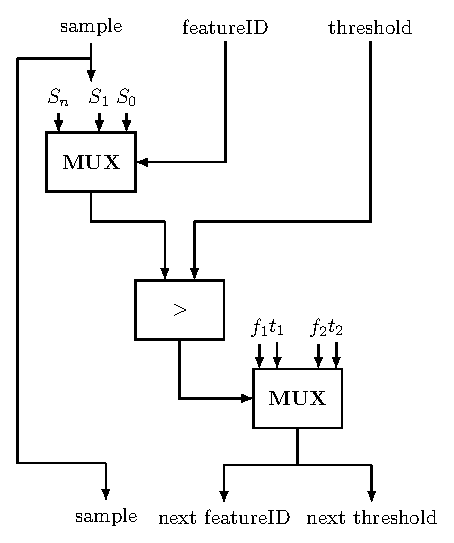
\includegraphics[width=0.60\textwidth]{images/decision_tree_node.pdf}
  \caption{Diagram representing the Boolean circuit of each node in a \ac{DT}.}
  \label{fig:DTNode}
\end{figure}


It is also important to mention that the trees that we used are always complete, \textit{i.e.} the number of nodes $n$ is always the maximum possible, and it can be defined as $n=2^{h+1}-1$, where $h$ is the \textit{height} of the tree. We can see in figure \ref{fig:ExpansionBinaryTrees} the implications of this expansion of the binary trees.

\begin{figure}[H]
	\centering
	\mbox{
		\subfigure[Original \ac{DT}.]{
		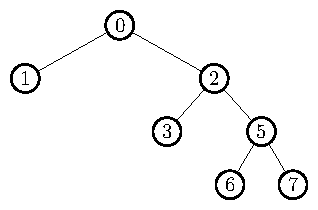
\includegraphics[width=0.40\textwidth]{images/decision_tree.pdf}
		\label{fig:Tree}
		}
		\subfigure[Complete \ac{DT}.]{
		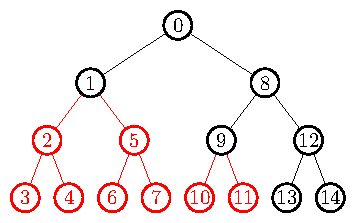
\includegraphics[width=0.40\textwidth]{images/decision_tree_complete.pdf}
		\label{fig:CompleteTree}
		}
	}
	\label{fig:ExpansionBinaryTrees}
	\caption{Expansion of binary trees.}
\end{figure}


In figure \ref{fig:Tree} we have a binary \ac{DT} with $height=3$ and with different path lengths to the leaves, depending on the branch of the tree taken, but on the tree in figure \ref{fig:CompleteTree}, all paths have the same length. With this, we can effectively hide the sparseness of the tree, which can leak relevant information about the original data. However, this solution increases exponentially the total amount of nodes that need to be evaluated, and that decreases performance significantly, as we will see in chapter \ref{ch:Evaluation}.
                


%%%%%%%%%%%%%%%%%%%%%%%%%%%%%%%%%%%%%%%%%%%%%%%%%%%
\subsection{Garbled Circuits and \textit{k}-means}
\label{ssec:GCandk-M}
%%%%%%%%%%%%%%%%%%%%%%%%%%%%%%%%%%%%%%%%%%%%%%%%%%%



As in the previous section, evaluating the \ac{k-M} algorithm in a privacy-preserving manner is similar to evaluating in the usual manner. We took the operations in the prediction step and transformed them in Boolean circuits, with logic gates such as multiplexers, adders, etc.

In figure \ref{fig:kmeans} we show how we designed the circuit to represent the \ac{k-M} prediction. The ED blocks represent the operations to perform the Euclidean distance between the sample and each centroid provided by the \ac{k-M} model. The ARGMIN block represent the operations needed to choose, between all the distances calculated, which of it is the smallest.


\begin{figure}[H]
  \centering
  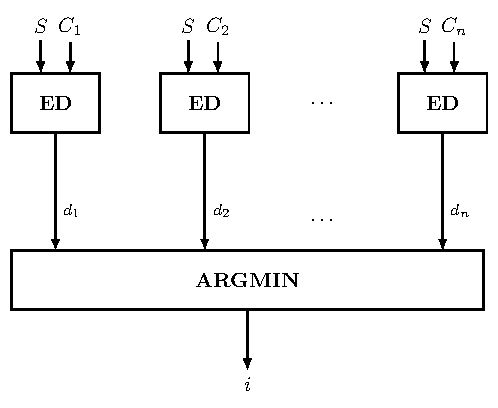
\includegraphics[width=0.60\textwidth]{images/k-means.pdf}
  \caption{Circuit representing the prediction of the \ac{k-M} algorithm.}
  \label{fig:kmeans}
\end{figure}


As we show in ref(evaluation-k.means), there is an exponential decrease in performance when the number of clusters increases, or the sample has a larger number of features. This is caused by the multiplications that are done calculating the Euclidean distance. Usually this is reason to use \ac{HE} instead, but the algorithm to implement comparisons is hard to implement \cite{blake2004strong}.\todo{is this justification enough?}




%%%%%%%%%%%%%%%%%%%%%%%%%%%%%%%%%%%%%%%%%%%%%%%%%%%
\subsection{Homomorphic Encryption and Support Vector Machines}
\label{ssec:GCandk-M}
%%%%%%%%%%%%%%%%%%%%%%%%%%%%%%%%%%%%%%%%%%%%%%%%%%%
\commentPT{
	Estas duas secções devem estar descritas como trabalho feito? (foi implementado pelo José Portelo)
	Ou ficam para future work? ou só mencionar noutro local da tese?

}
%%%%%%%%%%%%%%%%%%%%%%%%%%%%%%%%%%%%%%%%%%%%%%%%%%%
\subsection{Homomorphic Encryption and Logistic Regression}
\label{ssec:GCandk-M}
%%%%%%%%%%%%%%%%%%%%%%%%%%%%%%%%%%%%%%%%%%%%%%%%%%%